\begin{figure}[t]
\centering

\begin{subfigure}[b]{0.495\columnwidth}
\centering 
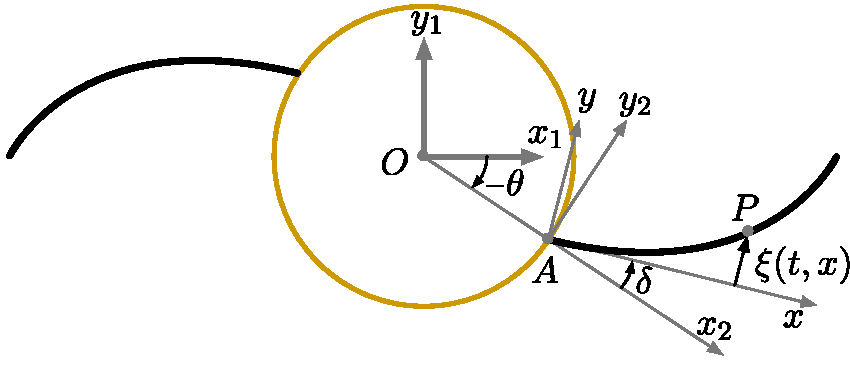
\includegraphics[height=1.2in]{../ch7/figures/coordinate-2}
\caption{Beam theory model.}\label{fig:ch7:coordinate}
\end{subfigure}%
\begin{subfigure}[b]{0.495\columnwidth}
\centering 
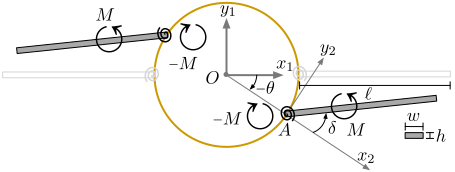
\includegraphics[height=1.2in]{../ch7/figures/prbdm-2}
\caption{Lumped parameter model.}\label{fig:ch7:prbdm}
\end{subfigure}%

\caption{Illustration of the two modeling approaches used to gain design insights. \label{fig:ch7:models}}
\end{figure} 